




\begin{figure}[t]

\centerline{
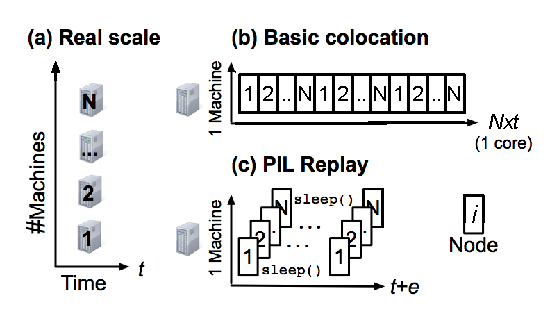
\includegraphics[height=1.75in]{F/ill/colo-hotos.eps}
%\includegraphics[height=1.75in]{F/empty.eps}
}

%\mycaption{fig-ill}{Real-scale testing, basic colocation, and scale check}{}
\mycaption{fig-ill}{Various scale-testing approaches}{The
left figure (a) illustrates a real-scale testing where the system/protocol
under test 
is deployed on $N$ machines, which illustratively takes $t$ time to complete.
%
The top figure (b) depicts a basic colocation where $N$ nodes
are packed into a single machine and exhibit CPU contention 
and context switching, which can take $N$$\times$$t$ time
to complete (in one-processor scenario).
%
The bottom figure (c) illustrates our 
processing illusion (PIL) as described in \sec\ref{sec-sck}. Here,
expensive functions are emulated with \ts{sleep()}, thus the test
time $t$$+$$e$ is similar to the real-scale testing. }


\end{figure}



